\chapter{Multiple Integrals}


In this chapter, we extend this powerful idea into higher dimensions using the 
tools of multiple integration. While single integration enables us to calculate
the area under a curve or the volume under a surface, multiple integration 
allows us to calculate volumes in three dimensions, and even hypervolumes in 
higher dimensions.

We start by discussing double integration, which allows us to find the volume 
under a surface in three dimensions. This method involves slicing the solid 
into infinitesimally thin disks, and summing the volumes of these disks.

Next, we'll cover triple integration, a tool that lets us find the volume of 
more complicated solids in three-dimensional space. The idea is similar to 
double integration, but instead of slicing the solid into disks, we slice it 
into infinitesimally small cubes.

To properly implement these techniques, we'll also discuss the different 
coordinate systems that can be used in multiple integration, such as 
rectangular, cylindrical, and spherical coordinates, and when it's advantageous
to use one system over another.

By the end of this chapter, you will have a deeper understanding of the 
techniques of multiple integration and how to apply them to find the volumes 
of various types of solids. The methods we study here will serve as a 
foundation for many topics in higher mathematics and physics, including 
electromagnetism, fluid dynamics, and quantum mechanics.

\section{Double Integrals}
[fixme intro paragraph]

\subsection{Over Rectangular Regions}
Suppose there is some function, $z = f(x,y)$, that is defined over the 
rectangular region, $R$, defined by $R = [a, b] \times [c,d] = \{(x,y)| a \leq 
x \leq b, c \leq y \leq d\}$, and $f$ is such that $f \geq 0$ for all $(x, y) 
\in \mathbb{R}$. Then the graph of $f$ is a surface that lies above the 
rectangular region, $R$ (see figure \ref{fig:f_on_R}). 

\begin{figure}[htbp]
    \centering
    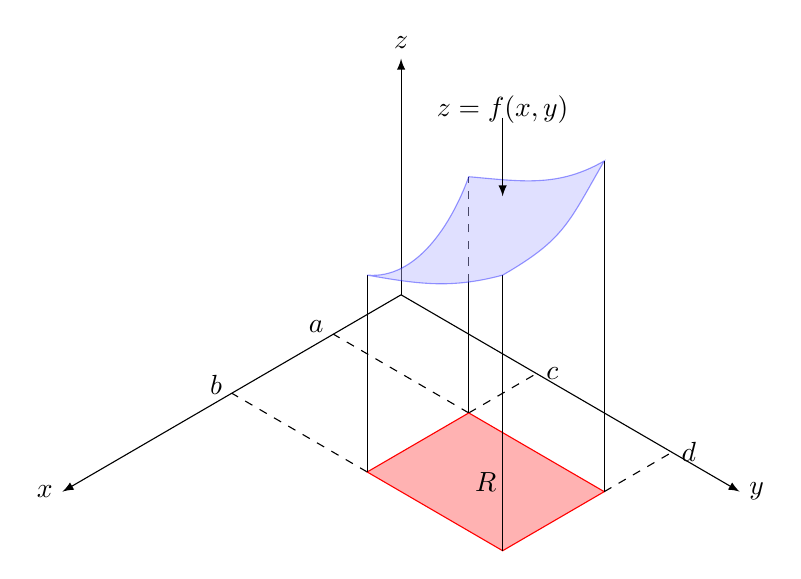
\begin{tikzpicture}[x = {(-0.86cm, -0.5cm)}, y = {(0.86cm, -0.5cm)}, 
    z = {(0cm, 1cm)}]
        \draw[-latex] (0,0,0) -- (5,0,0) node[left] {$x$};
        \draw[-latex] (0,0,0) -- (0,5,0) node[right] {$y$};
        \draw[-latex] (0,0,0) -- (0,0,3) node[above] {$z$};
        \draw[dashed] (1, 2, 0) -- (1, 0, 0) node[left, yshift = 0.1cm] {$a$};
        \draw[dashed] (2.5, 2, 0) -- (2.5, 0, 0) node[left, yshift = 0.1cm] 
        {$b$};
        \draw[dashed] (1, 2, 0) -- (0, 2, 0) node[right] {$c$};
        \draw[dashed] (1, 4, 0) -- (0, 4, 0) node[right] {$d$};
        \filldraw[draw = red, fill = red!30] (1, 2, 0) -- (2.5, 2, 0) -- 
        (2.5, 4, 0) -- (1, 4, 0) -- cycle;
        \node[] at (1.75, 3, 0) {$R$};
        \draw[] (2.5, 2, 0) -- (2.5, 2, 2.5);
        \draw[] (1, 2, 0) -- (1, 2, 1.66);
        \draw[dashed] (1, 2, 1.66) -- (1, 2, 3);
        \draw[] (2.5, 4, 0) -- (2.5, 4, 3.5);
        \draw[] (1, 4, 0) -- (1, 4, 4.2);
        \filldraw[draw = blue, fill = blue!30, opacity = 0.4] (2.5, 2, 2.5) 
        to[out = -5, in = -110, looseness = 0.9] (1, 2, 3) 
        to[out = -5, in = 210] (1, 4, 4.2) 
        to[out = 240, in = 30, looseness = 1.2] (2.5, 4, 3.5) 
        to[out = 195, in = -10] (2.5, 2, 2.5);
        \draw[-latex] (1, 2.5, 4) -- (1, 2.5, 3);
        \node[] at (1, 2.5, 4.1) {$z = f(x,y)$};
    \end{tikzpicture}
    \caption{The graph of $f$ over the region $R$}
    \label{fig:f_on_R}
\end{figure}

\subsection{Double Integrals over General Regions}

\section{Fubini's Theorem for Double Integrals}

\begin{mdframed}[style = important, frametitle = {Fubini's Theorem}]
If $f$ is continuous on the rectangle $R = \{ \left( x, y \right) | a \leq x 
\leq b, c \leq y \leq d \}$, then
$$\iint_R f(x,y)\,\,dA = \int_a^b \int_c^d f(x,y)\,dy\,dx = \int_c^d \int_a^b 
f(x,y)\,dx\,dy$$
\end{mdframed}

\begin{Exercise}[title={Applying Fubini's Theorem},label = fubini]
Rewrite the following double integrals as iterated integrals.
\begin{enumerate}
\item $\iint_R \frac{xy^2}{x^2 + 1}\,\,dA$, $R = \{(x,y)|0 \leq x \leq 1, -3 
\leq y \leq 3\}$
\item $\iint_R \frac{\sec{\theta}}{\sqrt{1 + t^2}}\,\,dA$, $R = \{(\theta, t) |
0 \leq \theta \leq \frac{\pi}{4}, 0 \leq t \leq 1 \}$
\end{enumerate}
\vspace{40mm}
\end{Exercise}

\begin{Answer}[ref = fubini]
\begin{enumerate}
\item $\int_0^1 \int_{-3}^3 \frac{xy^2}{x^2 + 1}\,dy\,dx$ OR $\int_{-3}^3 
\int_0^1 \frac{xy^2}{x^2 + 1}\,dx\,dy$
\item $\int_0^{\pi/4} \int_0^1 \frac{\sec{\theta}}{\sqrt{1 + t^2}}\,dt\,
d\theta$ OR $\int_0^1 \int_0^{\pi/4} \frac{\sec{\theta}}{\sqrt{1 + t^2}}\,
d\theta \,dt$
\end{enumerate}
\end{Answer}

\begin{Exercise}[title = {Evaluating Iterated Integrals}, label = iterate_1]
Evaluate the following iterated integrals.
\begin{enumerate}
\item $\int_0^1 \int_1^2 \left( x + e^{-y} \right)\,dx\,dy$
\item $\int_{-3}^3 \int_{0}^{\pi/2} \left( 2y + y^2 \cos{x} \right)\,dx\,dy$
\item $\int_0^3 \int_0^{\pi/2} t^2 \sin^3{\theta}\,d\theta\,dt$
\end{enumerate}
\vspace{100mm}
\end{Exercise}

\begin{Answer}[ref = iterate_1]
\begin{enumerate}
\item Answer: $\frac{5}{2} - \frac{1}{e}$. Solution: $\int_0^1 \int_1^2 \left( 
x + e^{-y} \right)\,dx\,dy = \int_0^1 \left( \frac{1}{2}x^2 + xe^{-y} \right)
|_{x=1}^{x=2}\,dy = \int_0^1 \left( 2 - \frac{1}{2} + 2e^{-y} - e^{-y} \right)
\,dy = \int_0^1 \left( \frac{3}{2} + e^{-y} \right)\,dy = \left[ \frac{3}{2}y 
- e^{-y} \right]_{y = 0}^{y = 1} = \left( \frac{3}{2}(1) - e^{-1} \right) - 
\left( \frac{3}{2}(0) - e^0 \right) = \frac{5}{2} - \frac{1}{e}$
\item Answer: $18$. Solution: $\int_{-3}^3 \int_{0}^{\pi/2} \left( 2y + y^2 
\cos{x} \right)\,dx\,dy = \int_{-3}^3 \left[ 2xy + y^2 \sin{x} \right]_{x = 0}^
{x = \pi/2}\,dy = \int_{-3}^3 \left[ \left( \pi y + y^2 \right) - \left( 0 + 0 
\right) \right]\,dy = \int_{-3}^3 \left( \pi y + y^2 \right)\,dy = \left[ 
\frac{\pi}{2}y^2 + \frac{1}{3}y^3 \right]_{y = -3}^{y = 3} = \left( \frac{\pi}{
2}(9) + \frac{1}{3}(27) \right) - \left( \frac{\pi}{2}(9) + \frac{1}{3}(-27) 
\right) = 9 - (-9) = 18$
\item Answer: $6$. Solution: $\int_0^3 \int_0^{\pi/2} t^2 \sin^3{\theta}\,
d\theta\,dt = \left( \int_0^3 t^2\,dt \right) \times \left( \int_0^{\pi/2} 
\sin^3{\theta}\,d\theta \right) = \left[ \frac{1}{3}t^3 \right]_{t = 0}^{t = 3}
\times \left( \int_0^{\pi/2} \sin{\theta} \sin^2{\theta}\,d\theta \right) = 9
\int_0^{\pi/2} \sin{\theta} \left( 1 - \cos^2{\theta} \right)\,d\theta = 9 
\left[ \int_0^{\pi/2} \sin{\theta}\,d\theta - \int_0^{\pi/2} \sin{\theta}
\cos^2{\theta}\,d\theta \right] = 9 \left[ \left( -\cos{\theta} \right) |_{
\theta = 0}^{\theta = \pi/2} + \left( \frac{1}{3}\cos^3{\theta} \right)|_{
\theta = 0}^{\theta = \pi/2} \right] = 9 \left[ -(-\cos{0}) + (-\frac{1}{3}
\cos^3{0}) \right] = 9 \left( 1 - \frac{1}{3} \right) = 9 \left( \frac{2}{3} 
\right) = 6$
\end{enumerate}
\end{Answer}

\begin{Exercise}[title={Using Polar Coordinates in Multiple Integration}, 
label=polarmulti]

\Question Use double integration to find the volume of the solid that lies under the surface $z = 4 - x^2 - y^2$ and above the $xy$-plane.

\end{Exercise}
\begin{Answer}[ref=polarmulti]

We are finding the volume of the solid that lies under the surface $z = 4 - x^2 - y^2$ and above the $xy$-plane.

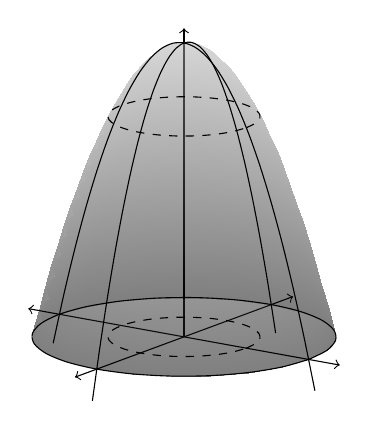
\begin{tikzpicture}
  \begin{axis}[
    view={35}{15},
    unit vector ratio=1 1 1,
    ticks = none,
    axis lines=middle,
    ymin=-2.5,
    ymax=2.5,
    xmax=2.5,
    xmin=-2.5,
    zmin=0,
    zmax=4.2,
    x axis line style=<->,
    y axis line style=<->,
    z axis line style=->,
    clip=false
  ]
    \addplot3[surf,shader=interp,domain=0:360,y domain=0:2, opacity=0.5,
    colormap={blackwhite}{color=(black) color=(black!30)}] ({y*cos(x)},
    {y*sin(x)},{4-y^2});
    \addplot3[samples y=0,domain=0:360,smooth]({2*cos(x)},  {2*sin(x)},0);
    \addplot3[samples y=0,domain=0:360,smooth,dashed]({cos(x)},  {sin(x)},0);
    \addplot3[samples y=0,domain=0:360,smooth,dashed]({cos(x)},  {sin(x)},3);
    \addplot3[samples y=0,domain=-2.1:2.1,smooth](0,  {x},{4 - x^2});
    \addplot3[samples y=0,domain=-2.1:2.1,smooth]({x},0, {4 - x^2});
  \end{axis}
\end{tikzpicture}

We can use polar coordinates to simplify the double integral. In polar coordinates, $x = r\cos(\theta)$ and $y = r\sin(\theta)$, so $x^2 + y^2 = r^2$. The volume under the surface and above the $xy$-plane is given by

\begin{equation}
V = \int \int (4 - r^2) r \, dr \, d\theta,
\end{equation}

where $r$ ranges from 0 to 2 (since $4 - r^2 \geq 0$ if $0 \leq r \leq 2$) and $\theta$ ranges from 0 to $2\pi$.

Hence,

\begin{align*}
V & = \int_{0}^{2\pi} \int_{0}^{2} (4r - r^3) \, dr \, d\theta \\
& = \int_{0}^{2\pi} \left[ 2r^2 - \frac{1}{4}r^4 \right]_{0}^{2} \, d\theta \\
& = \int_{0}^{2\pi} (8 - 4) \, d\theta \\
& = \int_{0}^{2\pi} 4 \, d\theta \\
& = \left[ 4\theta \right]_{0}^{2\pi} \\
& = 8\pi.
\end{align*}

So the volume of the solid is $8\pi$ cubic units.

\end{Answer}

\section{Triple Integrals}
